\documentclass[a5paper, 10pt]{article}

\usepackage{chirpstyle}
\usepackage{tkz-euclide}

\begin{document}

\section*{Circle Projection of Polygons}

\begin{definition}
    We call a polygon \textit{simple} if it is non-degenerate and non-intersecting.
\end{definition}

\begin{definition}
    Suppose we have a simple polygon \( P = \overline{A_1 A_2 \dots A_n} \) and a circle \( \omega \) with center \( O \). Define the \textit{circle projection} of \( P \) onto \( \omega \) by
    \[
        \Gamma (P, \omega) = \overline{B_1 B_2 \dots B_n}
    ,\]
    where \( B_k = \overrightarrow{OA_k} \cap \omega \).
\end{definition}

\begin{chirpbox}
\begin{problem}
    For every simple polygon \( P \), does there exist a circle \( \omega \) such that \( \Gamma (P, \omega) \) is convex and simple?
\end{problem}
\end{chirpbox}

\begin{figure}[!h]
    \centering
    \begin{tikzpicture}[scale=0.5]
        \tkzDefPoint(0,0){A};
        \tkzDefPoint(5,0){B};
        \tkzDefPoint(4,2){C};
        \tkzDefPoint(2,3){D};

        \tkzDefBarycentricPoint(A=1,B=1,C=1,D=1);
        \tkzGetPoint{O};

        \tkzDrawPolygon(A,B,C,D);
        \tkzDrawPoints(A,B,C,D,O);

        \tkzDefPoint(0, 4){Z};
        \tkzDefCircle(O,Z);
        \tkzDrawCircle(O,Z);

        \foreach \S in {A, B, C, D} {
            \tkzInterLC(O,\S)(O,Z);
            \tkzGetSecondPoint{\S'};
            \tkzDrawPoint(\S');

            \tkzDrawSegment[dotted](O,\S');
        }

        \tkzDrawPolygon(A',B',C',D');

        \tkzLabelPoint[below](A){\( A_1 \)};
        \tkzLabelPoint[below](B){\( A_2 \)};
        \tkzLabelPoint[above](C){\( A_3 \)};
        \tkzLabelPoint[above](D){\( A_4 \)};

        \tkzLabelPoint[left](A'){\( B_1 \)};
        \tkzLabelPoint[right](B'){\( B_2 \)};
        \tkzLabelPoint[right](C'){\( B_3 \)};
        \tkzLabelPoint[above](D'){\( B_4 \)};
        \tkzLabelPoint[above](O){\( O \)};
    \end{tikzpicture}
    \caption{A diagram showing the principle idea of the circle projection.}
\end{figure}

I'm not all too much of a geo guy (not by preference but just by what I've
experience in), but this was an interesting surprise of a problem that I
thought of while going to bed after USACO.

The key question one must tackle here is the case when \( P \) is concave (if
\( P \) is convex, then trivially the circle projection is convex too, although
I can't formalize this at the moment perhaps due to a lack of experience). We
can pretty assuredly answer this in the negative with a following example, so the goal narrows down to
being able to prove as such with a counterexample.

The reason why we can answer in the negative is contained in Figure 2. The
intuition behind this (intuition is all I really can give at this stage because
I'd need to think a whole lot more on how to actually formalize this; man I
really don't know enough geometry) is that, in order for the projected polygon
to be non-intersecting, the placement of the center \( O \) (the radius
actually does not matter at all as far as I can tell) needs to be such that the
clockwise/counterclockwise order of the vertices from \( O \) should correspond
to the actual order of the points (or like a modular shift of them but you
probably get the idea).

\begin{figure}
    \centering
    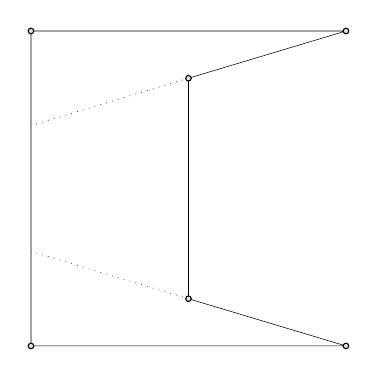
\begin{tikzpicture}[scale=2]
        \tkzDefPoint(0, 2){A};
        \tkzDefPoint(0, 0){B};
        \tkzDefPoint(2, 0){C};
        \tkzDefPoint(1, 0.3){D};
        \tkzDefPoint(1, 1.7){E};
        \tkzDefPoint(2, 2){F};

        \tkzInterLL(E,F)(A,B);
        \tkzGetPoint{N};

        \tkzDrawSegment[dotted](E,N);

        \tkzInterLL(C,D)(A,B);
        \tkzGetPoint{M};

        \tkzDrawSegment[dotted](D,M);

        \tkzDrawPolygon(A,B,C,D,E,F);
        \tkzDrawPoints(A,B,C,D,E,F);
    \end{tikzpicture}
    \caption{An example of a construction such that \( \Gamma(P, \omega) \) cannot possibly be non-intersecting.}
\end{figure}

When we have a concave dip in the shape, it closes off a region (given by the
extension of the segments connected to that concave dip point) that the point
must be in, otherwise we can't go in clockwise/counterclockwise order. By
creating two concave dips with disjoint regions, we immediately win.

Perhaps I shall attempt an actual proof when I learn more.


\end{document}
